\PassOptionsToPackage{dvipsnames}{xcolor}
\documentclass[aspectratio=169]{beamer}
\usetheme{Madrid}
\usecolortheme{default}
\usepackage{tikz}
\usetikzlibrary{positioning,shapes,arrows,arrows.meta,calc,fit}
\usepackage{graphicx}
\usepackage{booktabs}
\usepackage[utf8]{inputenc}
\usepackage[T1]{fontenc}
\usepackage{lmodern}
\usepackage{amsmath}
\usepackage{hyperref}
\usepackage{colortbl}
\usepackage{multirow}
\usepackage{array}
\usepackage{pifont}
\hypersetup{colorlinks=true, linkcolor=custompurple, urlcolor=custompurple}

% ── Colors ──────────────────────────────────────────────────
\definecolor{custompurple}{HTML}{4F2683}
\definecolor{lightpurple}{HTML}{8B5DB8}
\definecolor{palepurple}{HTML}{E8DEFF}
\definecolor{warmorange}{HTML}{E67E22}
\definecolor{lightorange}{HTML}{FAD7A0}
\definecolor{lightgray}{HTML}{F5F5F5}
\definecolor{darkred}{HTML}{C0392B}
\definecolor{medgray}{HTML}{AAAAAA}

% ── Beamer colors ───────────────────────────────────────────
\setbeamercolor{structure}{fg=custompurple}
\setbeamercolor{frametitle}{bg=white, fg=custompurple}
\setbeamercolor{background canvas}{bg=white}
\setbeamercolor{normal text}{fg=black}
\setbeamercolor{itemize item}{fg=custompurple}
\setbeamercolor{enumerate item}{fg=custompurple}
\setbeamercolor{block title}{bg=custompurple!20, fg=black}
\setbeamercolor{block body}{bg=custompurple!5}
\setbeamercolor{alerted text}{fg=custompurple}

% ── Templates ───────────────────────────────────────────────
\setbeamertemplate{navigation symbols}{}
\setbeamertemplate{headline}{}
\setbeamertemplate{frametitle}[default][center]
\setbeamerfont{frametitle}{series=\bfseries}

% ── Footer ──────────────────────────────────────────────────
\setbeamertemplate{footline}{
  \begin{tikzpicture}[remember picture,overlay]
    \fill[custompurple]
      (current page.south west)
      rectangle ([yshift=0.6cm]current page.south east);
    \node[anchor=west] at ([xshift=0.3cm,yshift=0.3cm]current page.south west){};
    \node[anchor=east, text=white, font=\footnotesize]
      at ([xshift=-0.3cm,yshift=0.3cm]current page.south east){
      \insertframenumber
    };
  \end{tikzpicture}
}

% ── Section cover macro ─────────────────────────────────────
\newcommand{\sectioncover}[1]{
{
\setbeamercolor{background canvas}{bg=custompurple}
\begin{frame}[plain]
  \begin{tikzpicture}[remember picture,overlay]
    \node[anchor=center, align=center, text width=0.85\paperwidth]
      at (current page.center)
      {\Huge\bfseries\color{white}#1};
    \fill[custompurple!70]
      (current page.south west)
      rectangle ([yshift=0.6cm]current page.south east);
    \node[anchor=east, text=white, font=\footnotesize]
      at ([xshift=-0.3cm,yshift=0.3cm]current page.south east){
      \insertframenumber
    };
  \end{tikzpicture}
\end{frame}
}}

% ============================================================
\begin{document}

% ─────────────────────────────────────────────────────────────
% TITLE SLIDE
% ─────────────────────────────────────────────────────────────
\begin{frame}[plain]
\begin{tikzpicture}[remember picture,overlay]
  \node[anchor=north] at ([yshift=-0.5cm]current page.north){
    
\includegraphics[height=1.2cm]{western.PNG}
  };
  \node[anchor=center, align=center, text width=0.9\paperwidth]
    at ([yshift=1.4cm]current page.center){
    {\fontsize{22}{28}\selectfont\bfseries\textcolor{custompurple}{Evaluating LLMs for Grade-Aware\\[0.2em]Educational Question Answering}}
  };
  \node[anchor=center, text width=0.85\paperwidth, align=center]
    at ([yshift=0.3cm]current page.center){
    {\normalsize A Controlled Ablation Study on ScienceQA}
  };
  \node[anchor=center, text width=0.85\paperwidth, align=center]
    at ([yshift=-1.2cm]current page.center){
    {\normalsize Western University}\\[0.5em]
    {\normalsize \textbf{ECE 9660 --- Large Language and Vision Models}}
  };
  \node[anchor=center, text width=0.85\paperwidth, align=center]
    at ([yshift=-3.0cm]current page.center){
    {\small\textcolor{medgray}{Presented by}}\\[0.2em]
    {\normalsize Ali Saab \quad\&\quad Nadine Charaf}
  };
  \fill[custompurple]
    (current page.south west)
    rectangle ([yshift=0.85cm]current page.south east);
  \node[anchor=west] at ([xshift=0.35cm,yshift=0.425cm]current page.south west){
    
\includegraphics[height=0.45cm]{western_eng.PNG}
  };
  \node[anchor=east, text=white]
    at ([xshift=-0.35cm,yshift=0.425cm]current page.south east){
    {\normalsize\insertframenumber}
  };
\end{tikzpicture}
\end{frame}

% ─────────────────────────────────────────────────────────────
% OUTLINE
% ─────────────────────────────────────────────────────────────
\begin{frame}{Presentation Outline}
\begin{columns}[T,totalwidth=\textwidth]
  \begin{column}{0.32\textwidth}
    \textbf{\textcolor{custompurple}{1.~Motivation}}
    \begin{itemize}\itemsep2pt\small
      \item The AI in education problem
      \item Grade-awareness gap
      \item Research questions
    \end{itemize}
  \end{column}
  \begin{column}{0.32\textwidth}
    \textbf{\textcolor{custompurple}{2.~Dataset \& Sampling}}
    \begin{itemize}\itemsep2pt\small
      \item ScienceQA overview
      \item Real examples
      \item Filter pipeline
    \end{itemize}
  \end{column}
  \begin{column}{0.32\textwidth}
    \textbf{\textcolor{custompurple}{3.~Methodology}}
    \begin{itemize}\itemsep2pt\small
      \item Ablation conditions
      \item Models tested
      \item Evaluation metrics
    \end{itemize}
  \end{column}
\end{columns}

\vspace{0.4cm}

\begin{columns}[T,totalwidth=\textwidth]
  \begin{column}{0.32\textwidth}
    \textbf{\textcolor{custompurple}{4.~Results}}
    \begin{itemize}\itemsep2pt\small
      \item Accuracy
      \item Grounding \& alignment
      \item Grade calibration
    \end{itemize}
  \end{column}
  \begin{column}{0.32\textwidth}
    \textbf{\textcolor{custompurple}{5.~Case Studies}}
    \begin{itemize}\itemsep2pt\small
      \item A success story
      \item A failure mode
    \end{itemize}
  \end{column}
  \begin{column}{0.32\textwidth}
    \textbf{\textcolor{custompurple}{6.~Conclusions}}
    \begin{itemize}\itemsep2pt\small
      \item Key findings
      \item Next steps
    \end{itemize}
  \end{column}
\end{columns}
\end{frame}

% ============================================================
\section{Motivation}
\sectioncover{Motivation}
% ============================================================

% ─────────────────────────────────────────────────────────────
\begin{frame}{AI Tutors Are Already in Classrooms}
\begin{columns}[T]
  \begin{column}{0.52\textwidth}
    \begin{block}{The Promise}
      \begin{itemize}\itemsep4pt
        \item LLMs can explain any concept on demand
        \item Available 24/7,  no teacher shortage problem
        \item Personalised: adapts tone, depth, examples
        \item Already used by millions of K--12 students
      \end{itemize}
   But, \\ Does the model \emph{actually} adapt to the student's level? Or does it always respond like a professor?
    \end{block}
  \end{column}
  \begin{column}{0.45\textwidth}
    \centering
    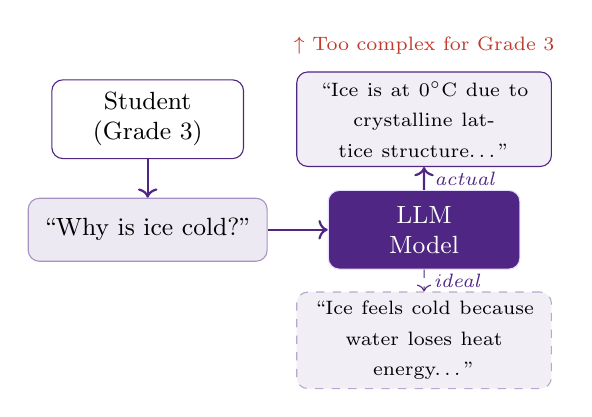
\begin{tikzpicture}[scale=0.78, every node/.style={font=\small}]
      % Student icon
      \node[draw=custompurple, rounded corners=4pt,
            fill=white, text width=2.2cm, align=center,
            minimum height=1cm] (student) at (0,0) {Student\\(Grade 3)};
      % Question arrow
      \node[draw=custompurple!50, rounded corners=4pt,
            fill=custompurple!10, text width=2.8cm, align=center,
            minimum height=0.8cm] (q) at (0,-1.8) {\small``Why is ice cold?''};
      \draw[->, thick, custompurple] (student) -- (q);
      % LLM box
      \node[
    draw=palepurple,
    rounded corners=4pt,
    fill=custompurple,
    text=white, % ← this makes the font white
    text width=2.2cm,
    align=center,
    minimum height=1cm
] (llm) at (4.5,-1.8) {LLM\\Model};
      \draw[->, thick, custompurple] (q) -- (llm);
      % Response options
      \node[draw=custompurple, rounded corners=4pt, fill=custompurple!8,
            text width=3cm, align=center,
            minimum height=0.9cm] (r1) at (4.5,0) {\scriptsize ``Ice is at 0$^\circ$C due to\\ crystalline lattice structure\ldots''};
      \node[draw=custompurple!40, rounded corners=4pt, fill=custompurple!8,
            text width=3cm, align=center, dashed,
            minimum height=0.9cm] (r2) at (4.5,-3.6) {\scriptsize ``Ice feels cold because\\ water loses heat energy\ldots''};
      \draw[->, thick, custompurple] (llm) -- node[right, font=\scriptsize]{\textit{actual}} (r1);
      \draw[->, dashed, custompurple] (llm) -- node[right, font=\scriptsize]{\textit{ideal}} (r2);
      % Grade label
      \node[font=\scriptsize, text=darkred] at (4.5, 1.2) {$\uparrow$ Too complex for Grade 3};
    \end{tikzpicture}
    \end{column}
    \end{columns}
    \begin{alertblock}{Grade-Awareness}
    Vocabulary- Reasoning depth-Examples used-  Response length
   
    \end{alertblock}


\end{frame}

% ───────────────────────────────────────────────────

% ─────────────────────────────────────────────────────────────
\begin{frame}{Problem Statement \& Research Questions}
\begin{columns}[T,onlytextwidth]

\begin{column}{0.42\textwidth}
\begin{block}{Problem Statement}
\footnotesize
Large language models lack awareness of a learner's grade level. 
Explanations may be too advanced, too simple, or pedagogically misaligned.
\end{block}

\vspace{0.1cm}

\begin{block}{Objective}
\footnotesize
Measure how \textbf{lecture context}, \textbf{hints}, and \textbf{grade metadata}
affect LLM accuracy and response quality.
\end{block}
\end{column}

\hfill

\begin{column}{0.52\textwidth}
\footnotesize
\textbf{Research Questions}


\begin{itemize}\itemsep4pt

\item \textbf{RQ1 -- Grounding}\\
How does providing a \textbf{lecture passage} affect accuracy?\\
\textit{Lecture vs parametric knowledge}

\item \textbf{RQ2 -- Hints}\\
What is the impact of adding a \textbf{pedagogical hint}?\\
\textit{Do hints reduce errors?}

\item \textbf{RQ3 -- Grade}\\
Does \textbf{grade metadata} produce age-appropriate explanations?\\
\textit{Do models adapt language?}

\item \textbf{RQ4 -- Models}\\
Do effects vary across \textbf{model size and architecture}?\\
\textit{Which models are more reliable?}

\end{itemize}

\end{column}

\end{columns}
\end{frame}

% ============================================================
\section{Dataset \& Sampling}
\sectioncover{Dataset \& Sampling}
% ============================================================

% ─────────────────────────────────────────────────────────────
\begin{frame}{ScienceQA: A K--12 Science Benchmark}
\begin{columns}[T]
  \begin{column}{0.52\textwidth}
    \begin{block}{What is ScienceQA?}
      \begin{itemize}\itemsep4pt
        \item Multiple-choice science questions from real curricula
        \item Covers elementary through middle school (Grades 1--12)
        \item Each question paired with an optional:
          \begin{itemize}\itemsep2pt
            \item \textbf{Lecture:} curriculum-aligned explanation
            \item \textbf{Hint:} pedagogical nudge for answering
            \item \textbf{Solution:} full worked answer
            \item \textbf{Image:} diagram or photo
          \end{itemize}
        \item Published by Lu et al.\ (NeurIPS 2022)
      \end{itemize}
    \end{block}
  \end{column}
  \begin{column}{0.45\textwidth}
    \centering
    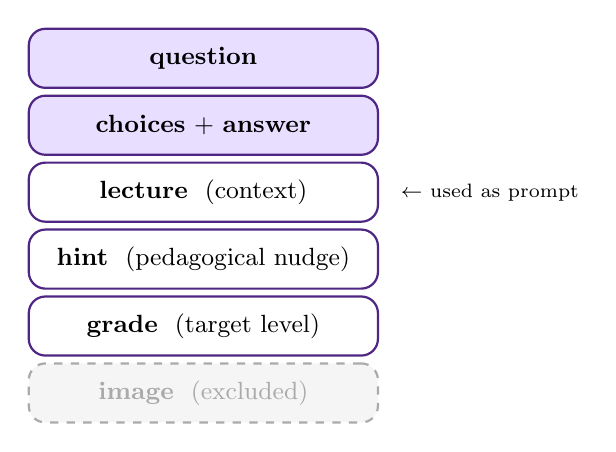
\begin{tikzpicture}[scale=0.85, every node/.style={font=\small}]
      % Fields diagram
      \node[draw=custompurple, thick, rounded corners=6pt,
            fill=palepurple, text width=4.2cm,
            align=center, minimum height=0.75cm] (q) at (0,0)
            {\textbf{question}};
      \node[draw=custompurple, thick, rounded corners=6pt,
            fill=palepurple, text width=4.2cm,
            align=center, minimum height=0.75cm] (ch) at (0,-1)
            {\textbf{choices} + \textbf{answer}};
      \node[draw=custompurple, thick, rounded corners=6pt,
            fill=white, text width=4.2cm,
            align=center, minimum height=0.75cm] (lec) at (0,-2)
            {\textbf{lecture}~~(context)};
      \node[draw=custompurple, thick, rounded corners=6pt,
            fill=white, text width=4.2cm,
            align=center, minimum height=0.75cm] (hint) at (0,-3)
            {\textbf{hint}~~(pedagogical nudge)};
      \node[draw=custompurple, thick, rounded corners=6pt,
            fill=white, text width=4.2cm,
            align=center, minimum height=0.75cm] (grade) at (0,-4)
            {\textbf{grade}~~(target level)};
      \node[draw=medgray, thick, dashed, rounded corners=6pt,
            fill=lightgray, text width=4.2cm,
            align=center, minimum height=0.75cm] (img) at (0,-5)
            {\textcolor{medgray}{\textbf{image}~~(excluded)}};
      % brace label
      \node[right=0.15cm of lec, font=\scriptsize, text=black] {$\leftarrow$ used as prompt};
    \end{tikzpicture}
  \end{column}
\end{columns}
\end{frame}

% ─────────────────────────────────────────────────────────────
\begin{frame}{ Example: Grade 3}
\begin{columns}[T]
  \begin{column}{0.52\textwidth}
    \begin{block}{Question (Grade 3)}
      \textbf{Which object has more thermal energy?}\\[6pt]
      \textbf{A.}~A cherry pie at 100$^\circ$F\\
      \textbf{B.}~A cherry pie at 85$^\circ$F\\[6pt]
      \textcolor{custompurple}{\textbf{Correct Answer: A}}
    \end{block}
    \vspace{0.2cm}
    \begin{alertblock}{Hint provided to model}
      \small ``The objects are identical except for their temperatures.''
    \end{alertblock}
  \end{column}
  \begin{column}{0.45\textwidth}
    \begin{block}{Lecture Excerpt}
      \small
      All solids, liquids, and gases are made of matter.
      Matter is made up of tiny particles that are always moving.
      The energy from the motion of these particles is called
      \textbf{thermal energy}.\\[4pt]
      Temperature measures how hot or cold matter is.
      If particles move faster, the temperature goes up.
    \end{block}
  
    
  \end{column}
\end{columns}
\end{frame}

% ─────────────────────────────────────────────────────────────
\begin{frame}{ Example: Grade 7}
\begin{columns}[T]
  \begin{column}{0.52\textwidth}
    \begin{block}{Question (Grade 7)}
      \textbf{What is the temperature of a pot of boiling water?}\\[6pt]
      \textbf{A.}~100$^\circ$F\\
      \textbf{B.}~100$^\circ$C\\[6pt]
      \textcolor{custompurple}{\textbf{Correct Answer: B}}
    \end{block}
    \vspace{0.2cm}
    \begin{alertblock}{Hint provided to model}
      \small ``Select the better estimate.''
    \end{alertblock}
  \end{column}
  \begin{column}{0.45\textwidth}
    \begin{block}{Lecture Excerpt}
      \small
      Temperature can be written with units of degrees Fahrenheit
      ($^\circ$F) or Celsius ($^\circ$C).\\[4pt]
      Reference points:\\
      $212^\circ$F / $100^\circ$C --- Water boils\\
      $98.6^\circ$F / $37^\circ$C --- Body temperature\\
      $32^\circ$F / $0^\circ$C --- Water freezes
    \end{block}
    
    
  \end{column}
\end{columns}
\end{frame}

% ─────────────────────────────────────────────────────────────
\begin{frame}{Sampling Strategy: From 4{,}241 to 375}

\begin{columns}[T]
  \begin{column}{0.52\textwidth}
    \textbf{Filter Pipeline}\\[6pt]
    \begin{tabular}{lrr}
      \toprule
      \textbf{Filter Step} & \textbf{Count} & \textbf{Kept}\\
      \midrule
      Full test split       & 4,241 & 100\%\\
      \rowcolor{palepurple}
      Remove image examples & 2,224 & 52.4\%\\
      Must have lecture     & 2,152 & 50.7\%\\
      \rowcolor{palepurple}
      Must have hint        & 742   & 18.3\%\\
      Must have grade       & 742   & 18.3\%\\
      \midrule
      \rowcolor{custompurple!15}
      \textbf{Eligible pool}& \textbf{742} & \textbf{18.3\%}\\
      \bottomrule
    \end{tabular}
    
    
  
  \end{column}
  \begin{column}{0.45\textwidth}
    \textbf{Stratified Random Sample}\\[6pt]
    \begin{tabular}{lcc}
      \toprule
      \textbf{Grade} & \textbf{Pool} & \textbf{Sampled}\\
      \midrule
      Grade 3 & 190 & 75\\
      Grade 4 & 183 & 75\\
      Grade 5 & 154 & 75\\
      Grade 6 & 140 & 75\\
      Grade 7 & 75 & 75\\
      \midrule
      \textbf{Total} & \textbf{742} & \textbf{375}\\
      \bottomrule
    \end{tabular}
    \vspace{0.3cm}
   
  \end{column}
\end{columns}
\begin{block}{Why these filters?}
\small
To ensure a fair comparison across all experimental settings, we restrict the dataset 
to examples that contain \textbf{lecture, hint, and grade information}. 

\end{block}
\end{frame}

% ─────────────────────────────────────────────────────────────
\begin{frame}{What Changes Across Conditions?}

\vspace{0.1cm}
\textit{Same question, different context windows given to the model:}

\vspace{0.2cm}
\begin{center}
\begin{tabular}{clccc}
\toprule
\textbf{Condition} & \textbf{Label} & \textbf{Lecture} & \textbf{Hint} & \textbf{Grade}\\
\midrule
\rowcolor{palepurple}
C0 & Question Only (Baseline) & --- & --- & ---\\
C1 & + Lecture & \checkmark & --- & ---\\
\rowcolor{palepurple}
C2 & + Hint & \checkmark & \checkmark & ---\\
C3 & + Grade & \checkmark & --- & \checkmark\\
\rowcolor{custompurple!20}
C4 & Full Context & \checkmark & \checkmark & \checkmark\\
\bottomrule
\end{tabular}
\end{center}




\begin{alertblock}{Example: same question, different prompt}
\small\texttt{C0 sees:~~ Question + Choices only}\\
\small\texttt{C4 adds:~~ Lecture | Hint | Grade 3}
\end{alertblock}
  

\end{frame}

% ============================================================
\section{Methodology}
\sectioncover{Methodology}
% ============================================================

% ─────────────────────────────────────────────────────────────
\begin{frame}{Models Under Evaluation}
\begin{columns}[T]
  \begin{column}{0.55\textwidth}
    \begin{tabular}{llcl}
      \toprule
      \textbf{Model} & \textbf{Type} & \textbf{Params} & \textbf{Via}\\
      \midrule
      \rowcolor{palepurple}
      LLaMA 3.2 & Local & 3B & Ollama\\
      LLaMA 3.1 & Local & 8B & Ollama\\
      \rowcolor{palepurple}
      Phi-4 Mini & Local & 3.8B & Ollama\\
      Mixtral 8$\times$7B & Local & $\sim$47B & Ollama\\
      \rowcolor{custompurple!15}
      Claude Haiku & Cloud & --- & API\\
      \bottomrule
    \end{tabular}
    \vspace{0.2cm}
    \begin{itemize}\itemsep4pt\small
      \item \textbf{Ollama:} runs models locally, zero API cost
      \item \textbf{Mixtral:} sparse mixture-of-experts, 13B active
    
    \end{itemize}
  \end{column}
  \begin{column}{0.42\textwidth}
    \begin{block}{Why these models?}
      \begin{itemize}\itemsep5pt\small
        \item Cover a spectrum of sizes (3B → 47B)
        \item Mix of architectures: dense, MoE, cloud
        \item Allow cost--performance trade-off analysis
        \item All instruction-tuned (follow prompt formats)
      \end{itemize}
    \end{block}
    
  \end{column}
\end{columns}
\end{frame}

% ─────────────────────────────────────────────────────────────
\begin{frame}{Metric 1: Answer Accuracy}
\begin{columns}[T]
  \begin{column}{0.52\textwidth}
      \textbf{Fraction of questions where the model's predicted answer
      matches the gold answer.}
    \vspace{0.3cm}
    \large
    \[
      \text{Acc} = \frac{1}{N}\sum_{i=1}^{N}\mathbf{1}\!\left[\hat{a}_i = a_i^*\right]
    \]
    \normalsize
    \vspace{0.3cm}
    \begin{tabular}{cl}
      $N$ & total examples\\
      $\hat{a}_i$ & model's predicted choice letter\\
      $a_i^*$ & gold answer letter\\
      $\mathbf{1}[\cdot]$ & indicator function (1 if true, 0 if false)
    \end{tabular}
  \end{column}
  \begin{column}{0.45\textwidth}
    \textbf{Why it matters:}
    \begin{itemize}\itemsep5pt
      \item Primary measure of correctness
      \item Directly interpretable (0--100\%)
      \item Computed per model $\times$ condition $\times$ grade
      \item Enables ablation comparison across C0--C4
    \end{itemize}
    \vspace{0.3cm}
    \begin{alertblock}{Example}
      \small
      Model says \texttt{Answer: A}\\
      Gold answer is \texttt{A}\\
      $\Rightarrow$ $\mathbf{1}[\hat{a}_i = a_i^*] = 1$ \textbf{(correct)}
    \end{alertblock}
  \end{column}
\end{columns}
\end{frame}

% ─────────────────────────────────────────────────────────────
\begin{frame}{Metric 2: Choice Consistency}
\begin{columns}[T]
  \begin{column}{0.52\textwidth}
   
      \textbf{Fraction of responses where the model produced a
     parseable answer letter (A, B, C, or D). }  
    \vspace{0.3cm}
    \large
    \[
      \text{Cons} = \frac{1}{N}\sum_{i=1}^{N}\mathbf{1}\!\left[\hat{a}_i \neq \varnothing\right]
    \]
    \normalsize
    \vspace{0.3cm}
    \begin{tabular}{cl}
      $\hat{a}_i \neq \varnothing$ & model produced a valid letter\\
      $\hat{a}_i = \varnothing$ & model failed to produce a choice
    \end{tabular}
  \end{column}
  \begin{column}{0.45\textwidth}
    \textbf{Why it matters:}
    \begin{itemize}\itemsep5pt
     
      \item A model that never outputs a letter cannot be scored
      \item Low consistency = instruction-following failure
     
    \end{itemize}
    \vspace{0.3cm}
    \begin{alertblock}{Parsing rule}
      \small Extract the first occurrence of\\
      \texttt{Answer: <letter>} from the response.\\
      If absent $\Rightarrow$ $\hat{a}_i = \varnothing$
    \end{alertblock}
  \end{column}
\end{columns}
\end{frame}

% ─────────────────────────────────────────────────────────────
\begin{frame}{Metric 3: Lecture Grounding}
\begin{columns}[T]
  \begin{column}{0.52\textwidth}
  
    \textbf{Does the model use the provided lecture when constructing its response?}

   
    \textbf{Semantic similarity (LG-Sem):}
    \[
      \text{LG-Sem}_i = \frac{\mathbf{e}(r_i)\cdot\mathbf{e}(\ell_i)}
                            {\|\mathbf{e}(r_i)\|\cdot\|\mathbf{e}(\ell_i)\|}
    \]
    \footnotesize $\mathbf{e}(\cdot)$ = sentence embedding (all-MiniLM-L6-v2)\normalsize

   
    \textbf{Keyword overlap (LG-Ovlp / ROUGE-1):}
    \[
      \text{LG-Ovlp}_i = \frac{|\text{tok}(\ell_i)\cap\text{tok}(r_i)|}{|\text{tok}(\ell_i)|}
    \]
    \footnotesize $\text{tok}(\cdot)$ = informative tokens (stopwords removed)\normalsize
  \end{column}
  \begin{column}{0.45\textwidth}
    \textbf{Why it matters:}
    \begin{itemize}\itemsep5pt
      \item Verifies that added lecture \textbf{actually influences} output
      \item LG-Sem: captures meaning similarity
      \item LG-Ovlp: captures literal vocabulary reuse
     
    \end{itemize}
    \vspace{0.2cm}
    \begin{alertblock}{Expected pattern}
      \small C0 (no lecture) $\to$ low LG-Ovlp\\
      C1/C2/C4 (lecture given) $\to$ higher LG-Ovlp
    \end{alertblock}
  \end{column}
\end{columns}
\end{frame}

% ─────────────────────────────────────────────────────────────
\begin{frame}{Metric 4: Hint Alignment}
\begin{columns}[T]
  \begin{column}{0.52\textwidth}

      \textbf{Does the model's response reflect the pedagogical hint
      that guided it toward the answer?}

    \vspace{0.2cm}
    \textbf{Semantic similarity (HA-Sem):}
    \[
      \text{HA-Sem}_i = \frac{\mathbf{e}(r_i)\cdot\mathbf{e}(h_i)}
                            {\|\mathbf{e}(r_i)\|\cdot\|\mathbf{e}(h_i)\|}
    \]
    \footnotesize $h_i$ = hint text for example $i$\normalsize

    \vspace{0.2cm}
    \textbf{Keyword overlap (HA-Ovlp / ROUGE-1):}
    \[
      \text{HA-Ovlp}_i = \frac{|\text{tok}(h_i)\cap\text{tok}(r_i)|}{|\text{tok}(h_i)|}
    \]
  \end{column}
  \begin{column}{0.45\textwidth}
    \textbf{Why it matters:}
    \begin{itemize}\itemsep5pt
      \item A good tutor \textbf{echoes the hint's strategy}
      \item High HA-Ovlp shows hint vocabulary appears in response
     
     
    \end{itemize}
    \vspace{0.2cm}
    \begin{alertblock}{Expected pattern}
      \small C0/C1 (no hint) $\to$ HA-Ovlp $\approx$ 0.24\\
      C2/C4 (hint given) $\to$ HA-Ovlp $\approx$ 0.51
    \end{alertblock}
  \end{column}
\end{columns}
\end{frame}

% ─────────────────────────────────────────────────────────────
\begin{frame}{Metric 5: Grade Calibration}
\begin{columns}[T]
  \begin{column}{0.52\textwidth}
    \textbf{Does the model's response reading level match the target grade?}
    \vspace{0.3cm}

    \begin{block}{Step 1 --- Score each response}
      \texttt{FKGL(response)} $\;\to\;$ a \textbf{grade-level number}\\[6pt]
      \small
      \begin{tabular}{ll}
        \textbf{Input}  & response text (any length)\\
        \textbf{Uses}   & sentence length + word syllable count\\
        \textbf{Output} & estimated school grade level (e.g.\ 9.2)\\
      \end{tabular}
    \end{block}

    \vspace{0.25cm}

    \begin{block}{Step 2 --- Measure calibration error}
      \texttt{error} $=$ \texttt{|FKGL(response) $-$ target\_grade|}\\[6pt]
      \small
      \begin{tabular}{ll}
        \textbf{Input}  & scored response + target grade (3--7)\\
        \textbf{Output} & grade-level gap (lower = better)\\
      \end{tabular}
    \end{block}
  \end{column}
  \begin{column}{0.45\textwidth}
    \textbf{Why it matters:}
    \begin{itemize}\itemsep5pt
      \item Low calibration error = response matches student level
      \item Separates \textbf{accuracy} from \textbf{appropriateness}
      \item A model can be 100\% correct but incomprehensible to a 3rd grader
    \end{itemize}
    \vspace{0.2cm}
    \begin{alertblock}{Expected pattern}
      \small C3/C4 (grade given) $\to$ lower error\\
      C0 (no grade) $\to$ model defaults to college level
    \end{alertblock}
  \end{column}
\end{columns}
\end{frame}

% ─────────────────────────────────────────────────────────────
\begin{frame}{Metric 6: Question Difficulty}
\begin{columns}[T]
  \begin{column}{0.52\textwidth}
 
      \textbf{Measures \textbf{intrinsic complexity} of the question text
      itself --- as a reference baseline for calibration.}
    
    \vspace{0.2cm}
    \textbf{Average Word Length (AWL):}
    \[
      \text{AWL}(q_i) = \frac{1}{|W(q_i)|}\sum_{w\in W(q_i)}|w|
    \]
   

    
    \textbf{Type-Token Ratio (TTR):}
    \[
      \text{TTR}(q_i) = \frac{|\text{unique tokens}|}{|\text{all tokens}|}
    \]
    \footnotesize lexical diversity (higher $\approx$ richer vocabulary)\normalsize
  \end{column}
  \begin{column}{0.45\textwidth}
    \textbf{Why it matters:}
    \begin{itemize}\itemsep5pt
      
      \item Provides context for interpreting accuracy differences: lower accuracy at G7 may reflect harder questions,
        not worse model performance
      \item Validates that grade labels are meaningful
    \end{itemize}
    \vspace{0.2cm}
    \begin{alertblock}{Expected pattern}
      \small G3 FKGL $<$ G7 FKGL (questions get harder)\\
      TTR should increase with grade
    \end{alertblock}
  \end{column}
\end{columns}
\end{frame}

% ============================================================
\section{Results}
\sectioncover{Results}
% ============================================================

% ─────────────────────────────────────────────────────────────
\begin{frame}{Answer Accuracy by Condition}
\begin{columns}[T]
  \begin{column}{0.46\textwidth}
    \centering
    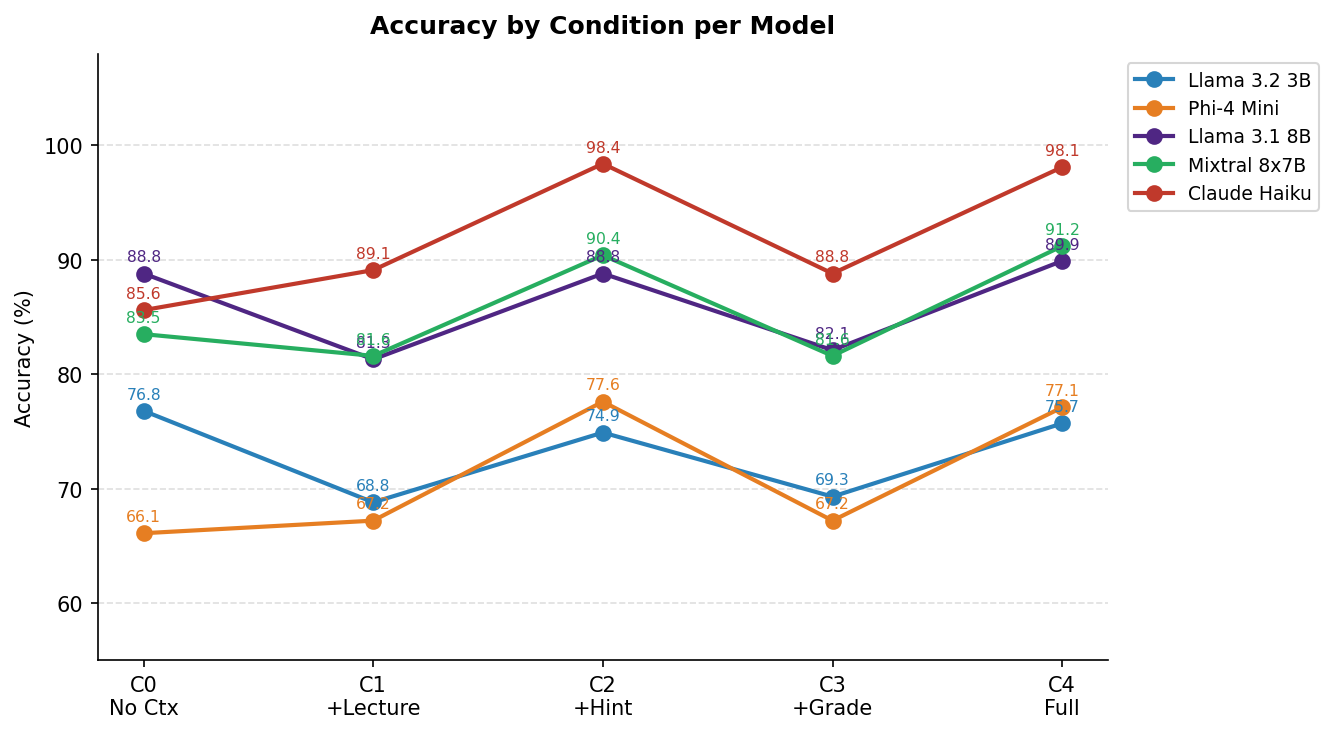
\includegraphics[width=\columnwidth]{fig2_accuracy_by_condition.png}
  \end{column}
  \begin{column}{0.51\textwidth}
    \small
    \begin{tabular}{lrrrrr}
      \toprule
      \textbf{Model} & \textbf{C0} & \textbf{C1} & \textbf{C2} & \textbf{C3} & \textbf{C4}\\
      \midrule
      Haiku  & .856 & .891 & \cellcolor{custompurple!20}.984 & .888 & \cellcolor{custompurple!15}.981\\
      L3.1-8B& .888 & .813 & .888 & .821 & \cellcolor{custompurple!10}.899\\
      L3.2-3B& .768 & .688 & .749 & .693 & .757\\
      Mixtral& .835 & .816 & \cellcolor{custompurple!15}.904 & .816 & \cellcolor{custompurple!20}.912\\
      Phi-4  & .661 & .672 & \cellcolor{custompurple!10}.776 & .672 & .771\\
      \midrule
      \textbf{Avg} & .802 & .776 & \cellcolor{custompurple!20}\textbf{.860} & .742 & \cellcolor{custompurple!15}\textbf{.864}\\
      \bottomrule
    \end{tabular}
    \vspace{0.3cm}
    \end{column}
\end{columns}
\begin{itemize}\itemsep4pt
      \item \textbf{C2 \& C4 consistently best:} hint drives gains
      \item \textbf{C1 $<$ C0:} lecture alone can hurt some models
      \item \textbf{Haiku:} massive jump from C0 (.856) to C2 (.984)
      \item \textbf{LLaMA 3.2 \& Phi-4:} modest gains from context
    \end{itemize}
\end{frame}

% ─────────────────────────────────────────────────────────────
\begin{frame}{Lecture Grounding \& Hint Alignment --- by Model}
\vspace{0.05cm}
\begin{columns}[T]
  \begin{column}{0.50\textwidth}
    \small\textbf{Lecture Grounding (LG-Ovlp)}\\
    {\footnotesize ROUGE-1 recall of lecture tokens in response.\\
    C0 = no lecture \quad C1 = lecture provided}
    \vspace{0.08cm}
    \begin{center}
    \renewcommand{\arraystretch}{1.2}
    \scriptsize
    \begin{tabular}{lccc}
      \toprule
      \textbf{Model} & \textbf{C0} & \textbf{C1} & \textbf{Gain}\\
      \midrule
      Claude Haiku  & 0.221 & \cellcolor{custompurple!20}\textbf{0.359} & $+$0.138\\
      Mixtral 8x7B  & 0.177 & \cellcolor{custompurple!15}0.311 & $+$0.134\\
      Phi-4 Mini    & 0.194 & \cellcolor{custompurple!15}0.349 & $+$0.155\\
      LLaMA 3.1 8B  & 0.172 & 0.289 & $+$0.117\\
      LLaMA 3.2 3B  & 0.162 & 0.262 & $+$0.100\\
      \midrule
      \textbf{Avg}  & 0.185 & \textbf{0.314} & \textbf{$+$0.129}\\
      \bottomrule
    \end{tabular}
    \end{center}
    \vspace{0.05cm}
    {\footnotesize All models are more grounded when lecture is provided ($+70\%$).}
  \end{column}
  \begin{column}{0.47\textwidth}
    \small\textbf{Hint Alignment (HA-Ovlp)}\\
    {\footnotesize ROUGE-1 recall of hint tokens in response.\\
    \textbf{Only for conditions with a hint: C2 and C4}}
    \vspace{0.08cm}
    \begin{center}
    \renewcommand{\arraystretch}{1.2}
    \scriptsize
    \begin{tabular}{lcc}
      \toprule
      \textbf{Model} & \textbf{C2} & \textbf{C4}\\
      \midrule
      Claude Haiku  & \cellcolor{custompurple!20}\textbf{0.628} & \cellcolor{custompurple!15}0.523\\
      Mixtral 8x7B  & \cellcolor{custompurple!15}0.531 & 0.476\\
      Phi-4 Mini    & 0.477 & 0.401\\
      LLaMA 3.1 8B  & 0.465 & 0.401\\
      LLaMA 3.2 3B  & 0.443 & 0.450\\
      \midrule
      \textbf{Avg}  & \textbf{0.509} & \textbf{0.450}\\
      \bottomrule
    \end{tabular}
    \end{center}
    \vspace{0.05cm}
    {\footnotesize Baseline (C0, no hint): HA-Ovlp $= 0.236$.\\
    With hint: avg $0.509$ --- \textbf{$+$116\% increase}.\\
    Claude Haiku most receptive (C2: 0.628).}
  \end{column}
\end{columns}
\end{frame}

% ─────────────────────────────────────────────────────────────
\begin{frame}{Grade Calibration Results --- by Model (C0 vs C4)}
\vspace{0.05cm}
{\footnotesize Target grade range: 3--7 \quad FKGL = Flesch--Kincaid Grade Level \quad Error = |FKGL $-$ target grade|}
\vspace{0.1cm}
\begin{center}
\renewcommand{\arraystretch}{1.3}
\small
\begin{tabular}{lrrrrr}
  \toprule
  \textbf{Model} & \textbf{C0 FKGL} & \textbf{C4 FKGL} & \textbf{C0 Error} & \textbf{C4 Error} & \textbf{Error $\downarrow$}\\
  \midrule
  Claude Haiku  & 11.6 & \cellcolor{custompurple!20}8.8  & 6.61 & \cellcolor{custompurple!20}3.88 & $-$41\%\\
  LLaMA 3.1 8B  & 11.5 & \cellcolor{custompurple!20}8.5  & 6.54 & \cellcolor{custompurple!20}3.54 & $-$46\%\\
  LLaMA 3.2 3B  & 12.3 & \cellcolor{custompurple!15}9.4  & 7.28 & \cellcolor{custompurple!15}4.41 & $-$39\%\\
  Mixtral 8x7B  & 11.2 & 10.1 & 6.16 & 5.07 & $-$18\%\\
  \rowcolor{darkred!8}
  Phi-4 Mini    & \textbf{18.8} & 12.6 & \textbf{13.82} & 7.58 & $-$45\%\\
  \bottomrule
\end{tabular}
\end{center}
\vspace{0.1cm}
\begin{columns}[T]
  \begin{column}{0.52\textwidth}
    \begin{itemize}\itemsep4pt\small
      \item All models respond to grade metadata --- FKGL drops for every model in C4
      \item \textbf{Haiku \& LLaMA 3.1} get closest to target range (FKGL 8.5--8.8)
      \item \textbf{Mixtral} least responsive ($-$18\% only)
      \item \textbf{Phi-4 Mini} starts as a severe outlier (18.8) but still improves $-$45\%
    \end{itemize}
  \end{column}
  \begin{column}{0.45\textwidth}
    \begin{block}{Key insight}
      \small Even with full grade context (C4), \textbf{no model reaches} the target reading level (FKGL 3--7).\\[4pt]
      Calibration and accuracy are \textbf{independent} --- a model can be correct but still write incomprehensibly for a 3rd grader.
    \end{block}
  \end{column}
\end{columns}
\end{frame}

% ============================================================
\section{Case Studies}
\sectioncover{Qualitative Case Studies}
% ============================================================

% ─────────────────────────────────────────────────────────────
\begin{frame}{Case Study: Same Question, Two Models --- Grade 4, C4}


  \textbf{Is the following trait inherited or acquired? Sasha is good at knitting hats.}\\
  A.~acquired \quad B.~inherited \quad \textcolor{custompurple}{\textbf{Correct: A}}\\
  \textit{Hint: ``People who can knit had to learn how to do it.''}

\begin{columns}[T]
  \begin{column}{0.48\textwidth}
    \begin{exampleblock}{Claude Haiku --- \textcolor{custompurple}{\checkmark} Correct}
      \scriptsize
      \textit{``\ldots According to the \textbf{lecture}, acquired traits are skills that people \textbf{learn} during their lives. The \textbf{hint tells us} that people who can knit had to \textbf{learn} how to do it. Sasha had to practice --- it is not something she was born knowing.''}
    \end{exampleblock}
    \renewcommand{\arraystretch}{1.1}
    \begin{tabular}{lr}
    
      LG-Ovlp (lecture used) & \cellcolor{custompurple!20}0.368\\
      HA-Ovlp (hint used)    & \cellcolor{custompurple!20}\textbf{1.000}\\
      FKGL of response       & 6.8\\
      Target grade           & 4\\
      Calibration error      & \cellcolor{custompurple!10}2.8\\
    \end{tabular}
  \end{column}
  \begin{column}{0.48\textwidth}
    \begin{alertblock}{Phi-4 Mini --- \textcolor{custompurple}{\checkmark} Correct (but\ldots)}
      \scriptsize
      \textit{``\ldots Being good at knitting hats is something Sasha \textbf{learned} to do over time through \textbf{practice}. This means it is an acquired trait because it was not passed down from her parents but was gained during her life by \textbf{practicing} the skill\ldots''}
    \end{alertblock}
    \renewcommand{\arraystretch}{1.1}
    \begin{tabular}{lr}
      
      LG-Ovlp (lecture used) & 0.368\\
      HA-Ovlp (hint used)    & \cellcolor{darkred!15}0.250\\
      FKGL of response       & 11.2\\
      Target grade           & 4\\
      Calibration error      & \cellcolor{darkred!15}\textbf{7.2}\\
    \end{tabular}
  \end{column}
\end{columns}
\vspace{0.1cm}
{\footnotesize Both models answer correctly --- but Phi-4 Mini barely uses the hint (HA-Ovlp: 0.25 vs 1.00) and writes at a college reading level for a Grade 4 student (FKGL 11.2 vs target 4).}
\end{frame}

% ─────────────────────────────────────────────────────────────
\begin{frame}{Case Study: Failure Mode --- Phi-4 Mini, Grade 3, C4}
\begin{columns}[T]
  \begin{column}{0.50\textwidth}
    
      \textbf{Which object has more thermal energy?}\\[4pt]
      A.~A cherry pie at 100$^\circ$F\\
      B.~A cherry pie at 85$^\circ$F\\[4pt]
      \textcolor{custompurple}{\textbf{Correct: A (100$^\circ$F)}}\\
      \textcolor{darkred}{\textbf{Phi-4 Predicted: B (85$^\circ$F) --- WRONG}}\\[2pt]
      \textit{Hint: ``The objects are identical except for their temperatures.''}
    \vspace{0.2cm}
    \begin{alertblock}{Phi-4 Mini Response (excerpt)}
      \scriptsize
      \texttt{Answer: B}\\[2pt]
      \textit{``Imagine you have two identical cherry pies\ldots The pie that's hotter has its tiny particles moving faster\ldots so it actually \textbf{feels colder}\ldots''}\\[3pt]
      \textcolor{darkred}{Correct concept, contradictory conclusion.}
    \end{alertblock}
  \end{column}
  \begin{column}{0.47\textwidth}
    \vspace{0.1cm}
    \renewcommand{\arraystretch}{1.25}
    \begin{tabular}{lr}
      \textbf{Correct?} & \cellcolor{darkred!20}\textbf{No}\\
      LG-Ovlp (lecture used) & 0.452\\
      HA-Ovlp (hint used)    & 0.500\\
      FKGL of response       & \cellcolor{darkred!20}13.3\\
      Target grade           & 3\\
      Calibration error      & \cellcolor{darkred!20}\textbf{10.3}\\
    \end{tabular}
    
    \begin{enumerate}\itemsep4pt\small
      \item \textbf{Wrong answer} --- logic error despite using lecture vocabulary
      \item \textbf{Grade mismatch} --- FKGL 13.3 for a Grade 3 student 
      \item \textbf{Contradictory reasoning} --- states correct physics, then inverts the conclusion
    \end{enumerate}
    \vspace{0.1cm}
   % {\footnotesize \textit{Accuracy alone cannot detect (2) or (3).}}
  \end{column}
\end{columns}
\end{frame}

% ============================================================
\section{Conclusions}
\sectioncover{Key Findings \& Next Steps}
% ============================================================

% ─────────────────────────────────────────────────────────────
\begin{frame}{Key Findings}
\begin{columns}[T]
  \begin{column}{0.48\textwidth}
    \textbf{\textcolor{custompurple}{Accuracy}}
    \begin{itemize}\itemsep4pt
      \item Pedagogical \textbf{hints} (C2, C4) are the most impactful
        context element --- +7 pp average over C0
      \item \textbf{Lecture alone} (C1) can \textit{hurt} accuracy for
        weaker models
      \item \textbf{Grade metadata} (C3) provides near-zero accuracy gain
     
    \end{itemize}

  
    \textbf{\textcolor{custompurple}{Grounding \& Alignment}}
    \begin{itemize}\itemsep4pt
      \item Hints are directly \textbf{absorbed} into responses

      \item Lecture grounding is modest 
    \end{itemize}
  \end{column}
  \begin{column}{0.48\textwidth}
    \textbf{\textcolor{custompurple}{Grade Calibration}}
    \begin{itemize}\itemsep4pt
      \item Without grade context, all models default to
        \textbf{college-level writing} (FKGL $\approx$ 13)
      \item Grade metadata reduces calibration error by \textbf{38\%}
      
      \item Accuracy and calibration are \textbf{independent}
    \end{itemize}

  \end{column}
\end{columns}
\end{frame}

% ─────────────────────────────────────────────────────────────
\begin{frame}{Next Steps}
\begin{columns}[T]
  \begin{column}{0.48\textwidth}
    \begin{block}{Expand Model Coverage}
      \begin{itemize}\itemsep5pt
        \item Test more cloud models:
          \begin{itemize}
            \item \textbf{Gemini} (Google, multi-grade instruction)
            \item \textbf{GPT-4o} (OpenAI, strong reasoning)
            \item \textbf{ChatGPT} (accessible baseline)
          \end{itemize}
     
        \item Instruction-tuned vs.\ base model comparison
      \end{itemize}
    \end{block}
  \end{column}
  \begin{column}{0.48\textwidth}
    \begin{block}{Improve Methodology}
      \begin{itemize}\itemsep5pt
        \item Extend to visual questions (multimodal)
        \item Human evaluation of response quality
        \item Fine-tune a small model on grade-conditioned data
        \item Automatic grade detection (no metadata needed)
        
      \end{itemize}
    \end{block}
  \end{column}
\end{columns}


\begin{block}{Broader Vision}
  \centering
  Build an open-source, grade-aware tutoring system that
  \textbf{automatically adapts} to any learner's level ---
  with no manual configuration required.
\end{block}
\end{frame}

% ─────────────────────────────────────────────────────────────
\begin{frame}[plain]
\begin{tikzpicture}[remember picture,overlay]
  \fill[custompurple] (current page.south west) rectangle (current page.north east);
  \node[anchor=center, align=center] at ([yshift=0.5cm]current page.center){
    {\Huge\bfseries\color{white}Questions?}\\[0.8cm]
    {\large\color{white!80}We welcome your thoughts and feedback.}
  };
  \fill[custompurple!70]
    (current page.south west)
    rectangle ([yshift=0.6cm]current page.south east);
  \node[anchor=west] at ([xshift=0.35cm,yshift=0.3cm]current page.south west){
    
\includegraphics[height=0.45cm]{western_eng.PNG}
  };
  \node[anchor=east, text=white, font=\footnotesize]
    at ([xshift=-0.3cm,yshift=0.3cm]current page.south east){
    \insertframenumber
  };
\end{tikzpicture}
\end{frame}

% ─────────────────────────────────────────────────────────────
\begin{frame}[plain]
\begin{tikzpicture}[remember picture,overlay]
  \fill[custompurple] (current page.south west) rectangle (current page.north east);
  \node[anchor=center, align=center] at ([yshift=1.0cm]current page.center){
    {\Huge\bfseries\color{white}Thank You!}\\[0.6cm]
    {\normalsize\color{white!80}Ali Saab \quad\&\quad Nadine Charaf}\\[0.3cm]
    {\normalsize\color{white!80}ECE 9660 --- Western University}
  };
  \node[anchor=center] at ([yshift=-1.8cm]current page.center){
    
\includegraphics[height=1.0cm]{western.PNG}
  };
  \fill[custompurple!70]
    (current page.south west)
    rectangle ([yshift=0.6cm]current page.south east);
  \node[anchor=west] at ([xshift=0.35cm,yshift=0.3cm]current page.south west){
    
\includegraphics[height=0.45cm]{western_eng.PNG}
  };
  \node[anchor=east, text=white, font=\footnotesize]
    at ([xshift=-0.3cm,yshift=0.3cm]current page.south east){
    \insertframenumber
  };
\end{tikzpicture}
\end{frame}

% 


\end{document}